\documentclass[11pt]{article}

% ---------- Packages ----------
\usepackage[utf8]{inputenc}
\usepackage[T1]{fontenc}
\usepackage[margin=1in]{geometry}
\usepackage{amsmath, amssymb}
\usepackage{booktabs}
\usepackage{array}
\usepackage{enumitem}
\usepackage{xcolor}
\usepackage{tikz}
\usetikzlibrary{shapes.geometric, arrows.meta, positioning, fit, backgrounds}
\usepackage{hyperref}
\hypersetup{colorlinks=true, linkcolor=blue, urlcolor=blue}

% ---------- TikZ styles ----------
\tikzset{
  block/.style   = {rectangle, draw, rounded corners, align=center,
                     fill=blue!8, minimum height=1cm, minimum width=2.4cm,
                     inner sep=6pt},
  group/.style   = {rectangle, draw, dashed, rounded corners, inner sep=10pt},
  arrow/.style   = {-{Stealth[length=3mm]}, thick},
  biarrow/.style = {{Stealth[length=3mm]}-{Stealth[length=3mm]}, thick},
}

\title{\textbf{The Absolute Basics (Read This First)}\\[4pt]
\large VLA Robot Project --- Foundations}
\author{Robotics + AI Mentor Notes}
\date{\today}

\begin{document}
\maketitle

\begin{abstract}
\noindent No setup, no commands. Just plain-language foundations so nothing later
feels like magic. Mental model of the whole project:
\textbf{Body (Isaac Sim), Nerves (ROS~2), Brain (our code $\rightarrow$ VLA).}
\end{abstract}

\tableofcontents
\bigskip
\hrule

% =====================================================================
\section{What is a robot (in our context)?}

A robot is a machine that \textbf{senses, thinks, and acts}:

\begin{center}
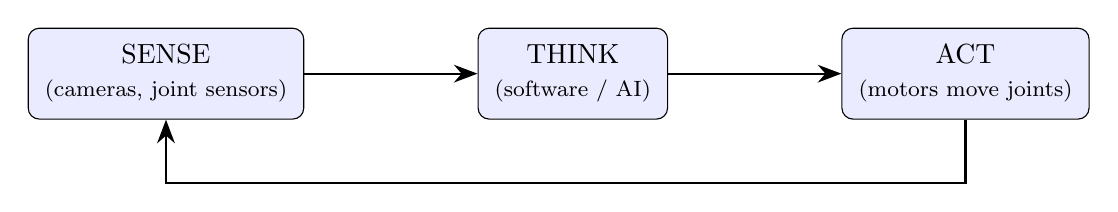
\begin{tikzpicture}[node distance=2.2cm]
  \node[block] (s) {SENSE\\{\footnotesize (cameras, joint sensors)}};
  \node[block, right=of s] (t) {THINK\\{\footnotesize (software / AI)}};
  \node[block, right=of t] (a) {ACT\\{\footnotesize (motors move joints)}};
  \draw[arrow] (s) -- (t);
  \draw[arrow] (t) -- (a);
  \draw[arrow] (a.south) -- ++(0,-0.8) -| (s.south);
\end{tikzpicture}
\end{center}

Our robot is a \textbf{robot arm} (a manipulator), like a human arm bolted to a table:
\begin{itemize}[leftmargin=*]
  \item \textbf{Links} = rigid segments (upper arm, forearm).
  \item \textbf{Joints} = movable connections (shoulder, elbow, wrist).
  \item \textbf{End-effector} = the ``hand'' / gripper at the tip.
\end{itemize}

Robot ``moving'' $=$ \textbf{motors rotate the joints}, repositioning the hand in space.

% =====================================================================
\section{What does ``control a robot'' actually mean?}

At the lowest level, controlling a robot $=$ \textbf{choosing the angle of each joint}.

A 6-joint arm has a joint-angle vector $\mathbf{q} \in \mathbb{R}^6$, for example:
\[
  \mathbf{q} =
  \begin{bmatrix}
    q_1 & q_2 & q_3 & q_4 & q_5 & q_6
  \end{bmatrix}^\top
  =
  \begin{bmatrix}
    0^\circ & -45^\circ & 90^\circ & 0^\circ & 45^\circ & 0^\circ
  \end{bmatrix}^\top .
\]
Change those numbers $\Rightarrow$ the arm moves.
\textbf{Every robot motion is ultimately a change in this vector $\mathbf{q}$.}

% =====================================================================
\section{Why simulation? What is Isaac Sim?}

Real robot arms are expensive, slow, and breakable. So we practice in a
\textbf{simulator} --- a physics-accurate virtual world.

\textbf{NVIDIA Isaac Sim} gives us:
\begin{itemize}[leftmargin=*]
  \item A virtual robot arm.
  \item Virtual cameras producing real-looking images.
  \item Virtual objects (red cube, box).
  \item Real physics (gravity, collisions, friction).
\end{itemize}

What we learn in sim mostly transfers to real robots later
--- \textbf{Phase 17, ``sim-to-real.''}

% =====================================================================
\section{What is ROS 2?}

The robot's software is \textbf{many small programs that must talk to each other}:
one reads the camera, one detects objects, one decides the action, one drives the motors.

\textbf{ROS~2 (Robot Operating System 2)} is the ``postal service'' connecting them.
Not an OS like Windows --- a \textbf{communication + tooling framework} for robots.

Core vocabulary (deep dive in Phase 3):
\begin{itemize}[leftmargin=*]
  \item \textbf{Node} = one small program (e.g., ``camera reader'').
  \item \textbf{Topic} = a named channel messages flow through (e.g., \texttt{/camera/image}).
  \item \textbf{Publisher} = a node that sends messages onto a topic.
  \item \textbf{Subscriber} = a node that listens to a topic.
  \item \textbf{Message} = the data itself (an image, a joint command, etc.).
\end{itemize}

\begin{center}
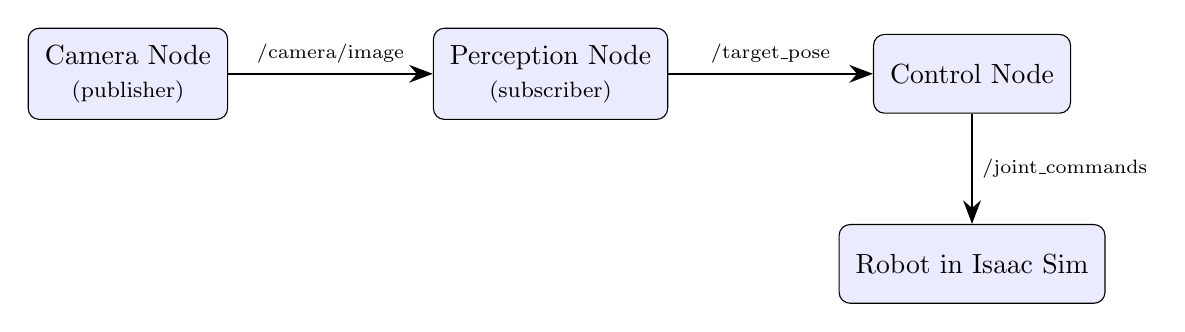
\begin{tikzpicture}[node distance=2.6cm]
  \node[block] (cam) {Camera Node\\{\footnotesize (publisher)}};
  \node[block, right=of cam] (per) {Perception Node\\{\footnotesize (subscriber)}};
  \node[block, right=of per] (ctrl) {Control Node};
  \node[block, below=1.4cm of ctrl] (rob) {Robot in Isaac Sim};
  \draw[arrow] (cam) -- node[above,font=\scriptsize]{/camera/image} (per);
  \draw[arrow] (per) -- node[above,font=\scriptsize]{/target\_pose} (ctrl);
  \draw[arrow] (ctrl) -- node[right,font=\scriptsize]{/joint\_commands} (rob);
\end{tikzpicture}
\end{center}

% =====================================================================
\section{What is a VLA --- in one sentence?}

\begin{itemize}[leftmargin=*]
  \item A \textbf{VLM} (Vision-Language Model): image $+$ text $\rightarrow$
        \textbf{describes} (``A red cube is on the table.'').
  \item A \textbf{VLA} (Vision-Language-Action model): image $+$ instruction
        $\rightarrow$ \textbf{acts} (outputs \emph{numbers that move the robot}).
\end{itemize}

\begin{center}
\fbox{\parbox{0.9\linewidth}{\centering
\textbf{VLA $=$ VLM $+$ the ability to produce robot actions.}\\
Turning understanding into motion is what makes robotics hard and interesting.}}
\end{center}

% =====================================================================
\section{How the pieces fit the final goal}

Goal: \textit{``Pick up the red object and put it in the box.''}

\begin{enumerate}[leftmargin=*]
  \item \textbf{Sense} --- cameras (Isaac Sim) send images via \textbf{ROS~2 topics}.
  \item \textbf{Think} --- software finds the red object and decides where to move.
  \item \textbf{Act} --- send joint-angle commands to the robot via ROS~2.
  \item \textbf{Repeat} --- look again, adjust (feedback loop).
\end{enumerate}

We first build step 2 with \textbf{classical hand-written logic} (Phase 7),
then later \textbf{replace the brain with a learned VLA} (Phases 9--16).

% =====================================================================
\section{The mental model to hold onto}

\begin{center}
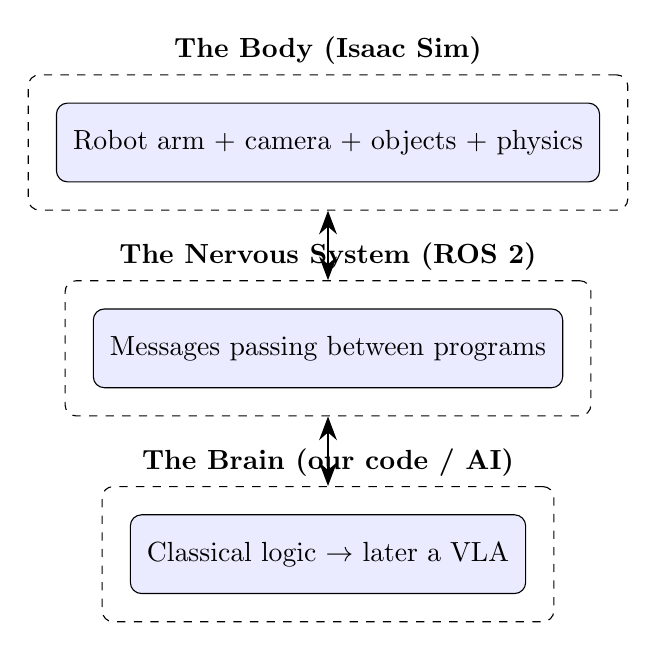
\begin{tikzpicture}[node distance=1.2cm]
  \node[block] (r) {Robot arm + camera + objects + physics};
  \begin{scope}[on background layer]
    \node[group, fit=(r), label=above:{\textbf{The Body (Isaac Sim)}}] (body) {};
  \end{scope}

  \node[block, below=1.6cm of r] (m) {Messages passing between programs};
  \begin{scope}[on background layer]
    \node[group, fit=(m), label=above:{\textbf{The Nervous System (ROS 2)}}] (nerves) {};
  \end{scope}

  \node[block, below=1.6cm of m] (c) {Classical logic $\rightarrow$ later a VLA};
  \begin{scope}[on background layer]
    \node[group, fit=(c), label=above:{\textbf{The Brain (our code / AI)}}] (brain) {};
  \end{scope}

  \draw[biarrow] (body) -- (nerves);
  \draw[biarrow] (nerves) -- (brain);
\end{tikzpicture}
\end{center}

\begin{itemize}[leftmargin=*]
  \item \textbf{Isaac Sim} = the body + world.
  \item \textbf{ROS~2} = the nervous system carrying signals.
  \item \textbf{Our code (eventually a VLA)} = the brain.
\end{itemize}

\begin{center}
\Large Three words: \textbf{Body, Nerves, Brain.}
\end{center}

% =====================================================================
\section*{Next step}
\addcontentsline{toc}{section}{Next step}
Once these basics feel clear, we return to \textbf{Phase 0}: verify the environment
(see \texttt{phase0\_environment.md}).

\end{document}
